\RequirePackage{fix-cm}
\documentclass{bmstu-sob}

% ------------------------------------------------------------
% Латиница
% ------------------------------------------------------------
% bmstu-sob использует XeLaTeX/LuaLaTeX и сам настраивает
% основной шрифт. Поэтому fontspec здесь повторно не подключаем.
%
% Латинские идентификаторы SQL:
% users, wallets, operations, operation_types
% поддерживаются непосредственно.

% ------------------------------------------------------------
% Нумерация разделов без привязки к главам
% ------------------------------------------------------------
\renewcommand{\thesection}{\arabic{section}}
\renewcommand{\thesubsection}{\arabic{section}.\arabic{subsection}}

% ------------------------------------------------------------
% Документ
% ------------------------------------------------------------
\begin{document}
	
	% ------------------------------------------------------------
	% Титульный лист
	% ------------------------------------------------------------
	\makereporttitle
{Платформенные решения для интеллектуального анализа больших данных}
{Компьютерные системы и сети}
{лабораторной работе №~2}
{Технология параллельных систем баз данных}
{Оптимизация запросов. Основы EXPLAIN в PostgreSQL. Индексация}
{1}
{Синдеев ~В.~А./ИУ6-13М}
{Григорьев~Ю.~А.}

\newpage
	% ============================================================
	% 1. ЦЕЛЬ РАБОТЫ
	% ============================================================
	
	\section{Цель работы}
	
	Формирование следующей компетенции: студент должен получить навыки работы с командой EXPLAIN. 
	Он также должен познакомиться с эффективными методами индексации в PostgreSQL
	
	\section{Основы EXPLAIN}
	
	Explain, Результат представлен на рисунке~\ref{fig:1}.
	
	\begin{figure}[htbp]
		\centering
		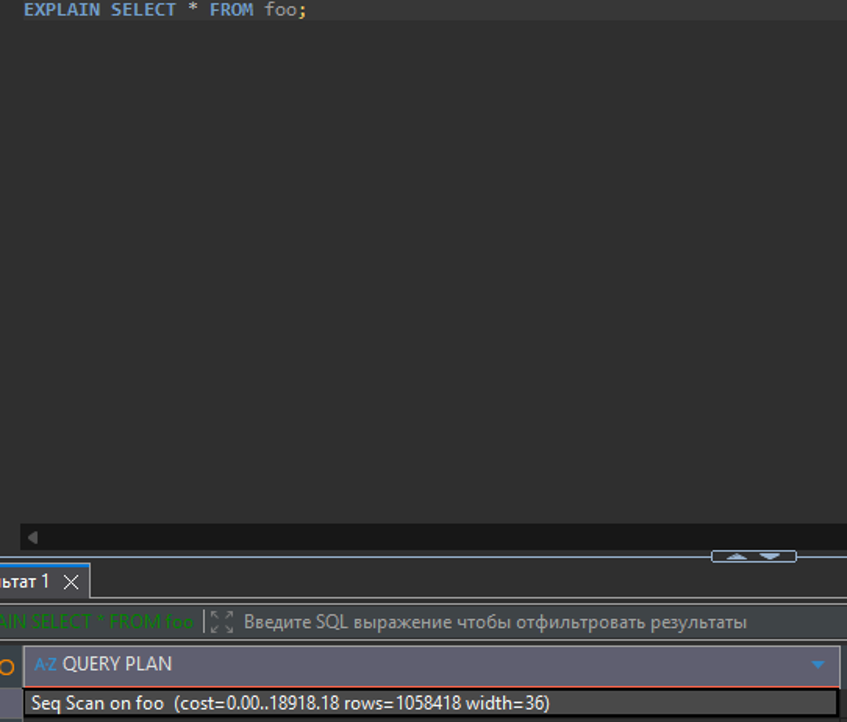
\includegraphics[
		width=0.6\textwidth
		]{img/1.png}
		\caption{Результат запроса}
		\label{fig:1}
	\end{figure}
	
	
	Добавили 10 строк, Результат представлен на рисунке~\ref{fig:2}.
	
	\begin{figure}[htbp]
		\centering
		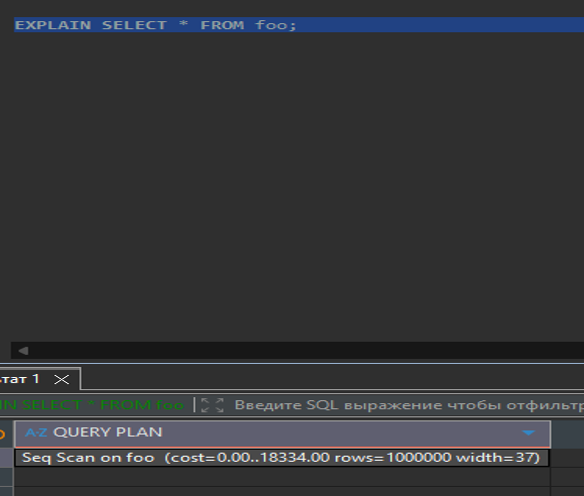
\includegraphics[
		width=0.6\textwidth
		]{img/2.png}
		\caption{План выполнения запроса + 10 строка}
		\label{fig:2}
	\end{figure}
	
	Данные планировщика не обновились, из-за малого количества добавленных строк. Можно обновить вручную.

	
	Выполнили команду ANALYZE foo, которая обновляет принудительно статистку для анализатора. Результат представлен на рисунке~\ref{fig:3}.
	
	\begin{figure}[htbp]
		\centering
		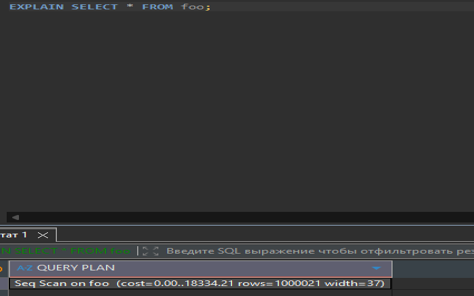
\includegraphics[
		width=0.6\textwidth
		]{img/3.png}
		\caption{План выполнения запроса после обновления данных у планировщика}
		\label{fig:3}
	\end{figure}
	
	Запрос вместе с analyze, мы получаем дополнительную информацию 
	Actual time реальное время полного прохождения по таблице 
	Rows количество строк пройденных в узле
	Loops Сколько раз выполнился узел 
	Planning time время построения плана
	Execution time время выполнения запроса. 
	
	
	Результат представлен на рисунке~\ref{fig:4}.
	
	\begin{figure}[htbp]
		\centering
		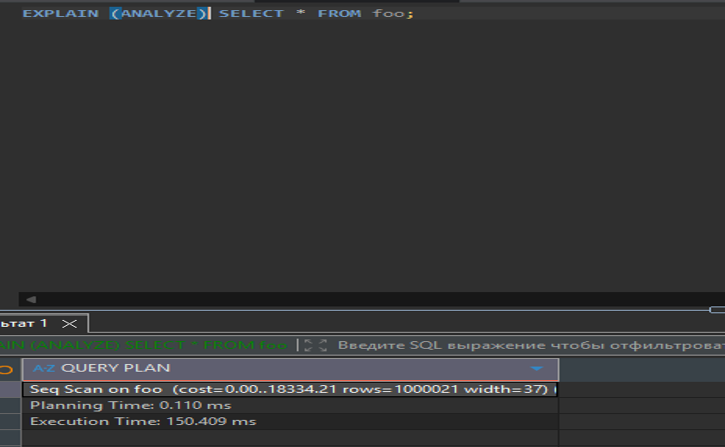
\includegraphics[
		width=0.6\textwidth
		]{img/4.png}
		\caption{План выполнения запроса с анализом}
		\label{fig:4}
	\end{figure}
	
	
	План выполнения с фильтром
	Rows строки, которые ожидаемо пройдут фильтр
	Filter: (c1 > 500) условие фильтра
	
	
	Результат представлен на рисунке~\ref{fig:5}.
	\begin{figure}[htbp]
		\centering
		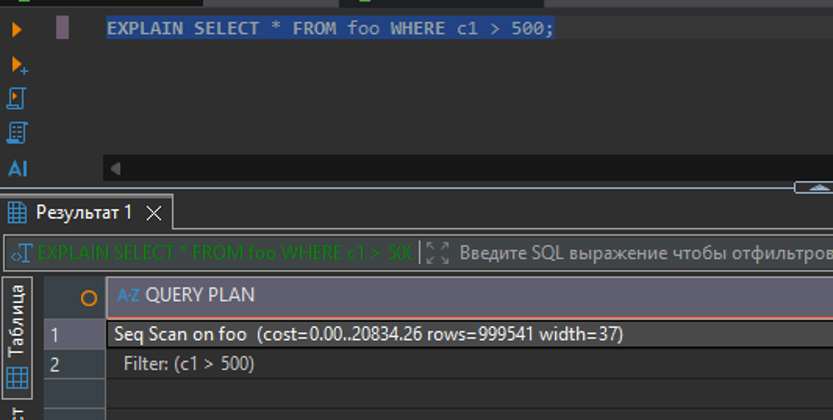
\includegraphics[
		width=0.6\textwidth
		]{img/5.png}
		\caption{План выполнения запроса с анализом}
		\label{fig:5}
	\end{figure}
	
	Создали индекс: 
	\begin{lstlisting}[language=SQL]
		create index idx_foo_c1 on foo (c1),
	\end{lstlisting}
	 Выполнили:
	\begin{lstlisting}[language=SQL]
	EXPLAIN SELECT * FROM foo WHERE c1 > 500;
	\end{lstlisting}
	Ничего не поменялось, условие откидывает много строк, Выполнили: 
	\begin{lstlisting}[language=SQL]
	EXPLAIN analyze SELECT * FROM foo WHERE c1 > 500;
	\end{lstlisting}
	результат: 
	\begin{lstlisting}[language=SQL]
	Seq Scan on foo  (cost=0.00..20834.26 rows=999495 width=37) (actual time=0.225..149.029 rows=999511 loops=1)
	Filter: (c1 > 500)
	Rows Removed by Filter: 510
	Planning Time: 0.099 ms
	Execution Time: 204.979 ms
	\end{lstlisting}
	
	Индекс будет использоваться при куске таблицы >~ 20\%, потому что это дешевле, при других обстоятельствах, чаще будет использоваться seq scan
	Вот пример запроса, который будет обрабатываться через индекс:
	
	Результат представлен на рисунке~\ref{fig:6}.
	
	\begin{lstlisting}[language=SQL]
	EXPLAIN SELECT * FROM foo WHERE c1 > 1000000;
	\end{lstlisting}
	
		\begin{figure}[htbp]
		\centering
		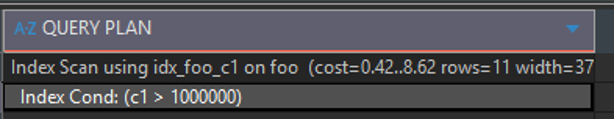
\includegraphics[
		width=0.6\textwidth
		]{img/6.png}
		\caption{План выполнения запроса с фильтром}
		\label{fig:6}
	\end{figure}
	
	
	Выполним запрос:
	\begin{lstlisting}[language=SQL]
	explain  SELECT * FROM foo
	WHERE c1 < 500 AND c2 LIKE 'abcd%';
	\end{lstlisting}
	
	результат:
	\begin{lstlisting}[language=SQL]
	Index Scan using idx_foo_c1 on foo  (cost=0.42..26.93 rows=1 width=37)
	Index Cond: (c1 < 500)
	Filter: (c2 ~~ 'abcd%'::text)
	\end{lstlisting}


	
	\subsection{}
	Сначала быстро за счет индекса отбрасываем не нужные строчки, далее ищем совпадения в подстроке 
		Выполним запрос: 
	\begin{lstlisting}[language=SQL]
	explain  SELECT * FROM foo
	WHERE c2 LIKE 'abcd%';
	Gather  (cost=1000.00..14552.44 rows=100 width=37)
	Workers Planned: 2
	->  Parallel Seq Scan on foo  (cost=0.00..13542.44 rows=42 width=37)
	Filter: (c2 ~~ 'abcd%'::text)
	\end{lstlisting}
	
	Нет индекса поэтому последовательно
	создадим индекс для c2: 
	\begin{lstlisting}[language=SQL]
create index idx_foo_c2 on foo (c2 text_pattern_ops)
	\end{lstlisting}
	
	Выполним запрос:
	\begin{lstlisting}[language=SQL]
explain  SELECT * FROM foo WHERE c2 LIKE 'abcd%';
	\end{lstlisting}
	
	Результат:
	\begin{lstlisting}[language=SQL]
Index Scan using idx_foo_c2 on foo  (cost=0.42..8.45 rows=100 width=37)
Index Cond: ((c2 ~>=~ 'abcd'::text) AND (c2 ~<~ 'abce'::text))
Filter: (c2 ~~ 'abcd%'::text)
	\end{lstlisting}
	
	Теперь мы наглядно видим что используется индекс для работы с текстовыми паттернами
	
	\subsection{Удаление индекса c1}
	выполним команду: 
	\begin{lstlisting}[language=SQL]
		drop index idx_foo_c1
	\end{lstlisting}
	
	результат:
	\begin{lstlisting}[language=SQL]
Gather Merge  (cost=63790.40..161021.35 rows=833350 width=37) (actual time=111.264..276.359 rows=1000021 loops=1)
Workers Planned: 2
Workers Launched: 2
->  Sort  (cost=62790.37..63832.06 rows=416675 width=37) (actual time=100.106..135.931 rows=333340 loops=3)
Sort Key: c1
Sort Method: external merge  Disk: 16640kB
Worker 0:  Sort Method: external merge  Disk: 14408kB
Worker 1:  Sort Method: external merge  Disk: 15136kB
->  Parallel Seq Scan on foo  (cost=0.00..12500.75 rows=416675 width=37) (actual time=0.039..20.431 rows=333340 loops=3)
Planning Time: 0.735 ms
Execution Time: 310.805 ms
	\end{lstlisting}
	Прочитает всю таблицу, отсортирует все строки из памяти или диска
	
	\subsection{Увеличим объем памяти до 200мб}
	
	выполним команду:
	\begin{lstlisting}[language=SQL]
set_work_mem to “200MB”
	\end{lstlisting}
	
	\subsection{Повторим запрос}
	
	\begin{lstlisting}[language=SQL]
Sort  (cost=117994.30..120494.35 rows=1000021 width=37) (actual time=310.384..343.105 rows=1000021 loops=1)
Sort Key: c1
Sort Method: quicksort  Memory: 102703kB
->  Seq Scan on foo  (cost=0.00..18334.21 rows=1000021 width=37) (actual time=0.035..53.149 rows=1000021 loops=1)
Planning Time: 0.196 ms
Execution Time: 382.072 ms
	\end{lstlisting}
	Теперь сортировка выполняется в озу
	
	\subsection{Создание индекса для c1}
	
	Создадим индекс для поля \texttt{c1}.
	
	\begin{lstlisting}[language=SQL]
		
		
		CREATE INDEX idx_foo_c1 ON foo (c1);
	\end{lstlisting}
	
	
	Повторим запрос:
	
	\begin{lstlisting}[language=SQL]
		
		
		EXPLAIN ANALYZE SELECT * FROM foo ORDER BY c1;
	\end{lstlisting}
	
	
	Результат:
	
	\begin{lstlisting}[language=SQL]
Index Scan using idx_foo_c1 on foo
(cost=0.42..34317.74 rows=1000021 width=37)
(actual time=1.912..190.837 rows=1000021 loops=1)
Planning Time: 0.685 ms
Execution Time: 220.796 ms
	\end{lstlisting}
	
	
	Данные читаются в уже отсортированном виде за счет индекса.
	
	\subsection{Создание таблицы bar}
	
	Создадим таблицу \texttt{bar}:
	
	\begin{lstlisting}[language=SQL]
	CREATE TABLE bar (
		c1 integer,
		c2 boolean
		);
	\end{lstlisting}
	
	
	Заполним таблицу данными:
	
	\begin{lstlisting}[language=SQL]
	INSERT INTO bar
		SELECT i, i % 2 = 1
		FROM generate_series(1, 500000) AS i;
	\end{lstlisting}
	
	
	\subsection{JOIN без индекса}
	
	Выполним соединение таблиц без индекса:
	
	\begin{lstlisting}[language=SQL]
EXPLAIN ANALYZE
SELECT * FROM foo JOIN bar ON foo.c1 = bar.c1;
	\end{lstlisting}
	
	
	Результат:
	
	\begin{lstlisting}[language=SQL]
Hash Join
(cost=13463.00..40547.29 rows=500000 width=42)
(actual time=100.039..506.343 rows=500010 loops=1)
Hash Cond: (foo.c1 = bar.c1)
-> Seq Scan on foo
(cost=0.00..18334.21 rows=1000021 width=37)
(actual time=0.006..52.525 rows=1000021 loops=1)
-> Hash
(cost=7213.00..7213.00 rows=500000 width=5)
(actual time=99.728..99.730 rows=500000 loops=1)
Buckets: 524288  Batches: 1  Memory Usage: 22163kB
-> Seq Scan on bar
(cost=0.00..7213.00 rows=500000 width=5)
(actual time=0.007..24.519 rows=500000 loops=1)
Planning Time: 0.393 ms
Execution Time: 520.569 ms
	\end{lstlisting}
	
	
	В данном случае PostgreSQL использует \texttt{Hash Join}.
	
	Сначала читается меньшая таблица \texttt{bar}, после чего по ней строится хеш-таблица в памяти.
	Затем читается большая таблица \texttt{foo}.
	Для каждой строки таблицы \texttt{foo} выполняется поиск совпадения в хеш-таблице по полю \texttt{c1}.
	
	\subsection{JOIN с индексом}
	
	Создадим индекс для поля \texttt{c1} таблицы \texttt{bar}:
	
	\begin{lstlisting}[language=SQL]
CREATE INDEX idx_bar_c1 ON bar (c1);
	\end{lstlisting}
	
	
	Повторим запрос из предыдущего пункта:
	
	\begin{lstlisting}[language=SQL]
	EXPLAIN ANALYZE SELECT * FROM foo
JOIN bar ON foo.c1 = bar.c1;
	\end{lstlisting}
	
	
	Получим следующий план выполнения:
	
	\begin{lstlisting}[language=SQL]
	Merge Join
	(cost=2.46..40019.70 rows=500000 width=42)
	(actual time=0.118..481.829 rows=500010 loops=1)
	Merge Cond: (foo.c1 = bar.c1)
-> Index Scan using idx_foo_c1 on foo
	(cost=0.42..34317.74 rows=1000021 width=37)
	(actual time=0.030..68.980 rows=500011 loops=1)
-> Index Scan using idx_bar_c1 on bar
	(cost=0.42..15212.42 rows=500000 width=5)
	(actual time=0.016..290.617 rows=500010 loops=1)	
	Planning Time: 0.686 ms
	Execution Time: 498.625 ms
	\end{lstlisting}
	
	
	Теперь PostgreSQL читает таблицу \texttt{foo} уже в отсортированном порядке
	с помощью индекса \texttt{idx\_foo\_c1}.
	
	Одновременно таблица \texttt{bar} читается в отсортированном порядке
	с помощью индекса \texttt{idx\_bar\_c1}.
	
	Поскольку оба потока отсортированы по полю \texttt{c1}, PostgreSQL
	сливает их как два отсортированных списка. В результате используется
	алгоритм \texttt{Merge Join}.
	
	\subsection{Очистка кэша}
	
	Для проверки влияния кэша необходимо очистить кэш операционной системы.
	Для этого были выполнены следующие команды:
	
	\begin{lstlisting}[language=bash]
sudo service postgresql stop
		sudo sync
		sudo su root
		echo 3 > /proc/sys/vm/drop_caches
		exit
		sudo service postgresql start
		sudo -u admin psql lab2
	\end{lstlisting}
	
	
	После этого выполним запрос:
	
	\begin{lstlisting}[language=SQL]
EXPLAIN (ANALYZE, BUFFERS) SELECT * FROM foo;
	\end{lstlisting}
	
	
	Полученные результаты можно представить следующим образом:
	
	\begin{center}
		\begin{tabular}{|c|c|c|c|}
			\hline
			Запуск & shared\_hit & shared\_read & Комментарий \\
			\hline
			1-й & $\approx 0$ & много & Данные читаются с диска \\
			\hline
			2-й & растёт & уменьшается & Часть данных уже в кэше PostgreSQL \\
			\hline
			3-й & почти всё & почти 0 & Почти всё берётся из shared buffers \\
			\hline
		\end{tabular}
	\end{center}
	
	\texttt{shared\_hit} --- блоки, полученные из кэша PostgreSQL.
	
	\texttt{shared\_read} --- блоки, прочитанные с диска.
	
	Таким образом, повторное выполнение запроса позволяет увидеть влияние
	кэширования данных на работу PostgreSQL.
	
	\section{Эффективные методы индексации в PostgreSQL}
	
	Создадим таблицу \texttt{users} и добавим необходимые индексы.
	После этого заполним таблицу данными.
	
	\subsection{Индекс для поиска по фрагменту текста ILIKE}
	
	Выполним запрос:
	
	\begin{lstlisting}[language=SQL]
EXPLAIN
SELECT count(*)
FROM users
WHERE email ILIKE '%yandex.ru%';
	\end{lstlisting}
	
	
	До создания индекса PostgreSQL использует последовательное сканирование таблицы:
	
	\begin{lstlisting}[language=SQL]
Finalize Aggregate  (cost=16924.12..16924.13 rows=1 width=8)
->  Gather  (cost=16923.90..16924.11 rows=2 width=8)
Workers Planned: 2
->  Partial Aggregate  (cost=15923.90..15923.91 rows=1 width=8)
->  Parallel Seq Scan on users  (cost=0.00..15650.33 rows=109428 width=0)
Filter: (email ~~* '%yandex.ru%'::text)
	\end{lstlisting}
	
	
	Для эффективного поиска по фрагменту текста подключим расширение
	\texttt{pg\_trgm}:
	
	\begin{lstlisting}[language=SQL]
CREATE EXTENSION IF NOT EXISTS pg_trgm;
	\end{lstlisting}
	
	
	Расширение \texttt{pg\_trgm} добавляет поддержку триграмм --- разбиения
	строки на последовательности из трёх символов.
	
	Создадим GIN-индекс:
	
	\begin{lstlisting}[language=SQL]
CREATE INDEX idx_users_email_trgm ON users USING gin (email gin_trgm_ops);
	\end{lstlisting}
	
	
	После создания индекса повторим запрос.
	
	В результате используется следующая последовательность операций:
	\begin{lstlisting}[language=SQL]
Finalize Aggregate  (cost=15562.98..15562.99 rows=1 width=8) (actual time=658.663..671.236 rows=1 loops=1)
->  Gather  (cost=15562.77..15562.98 rows=2 width=8) (actual time=657.489..671.218 rows=3 loops=1)
Workers Planned: 2
Workers Launched: 2
->  Partial Aggregate  (cost=14562.77..14562.78 rows=1 width=8) (actual time=594.369..594.371 rows=1 loops=3)
->  Parallel Bitmap Heap Scan on users  (cost=2479.35..14289.20 rows=109428 width=0) (actual time=134.492..582.651 rows=83239 loops=3)	Recheck Cond: (email ~~* '%yandex.ru%'::text)
Heap Blocks: exact=3456
->  Bitmap Index Scan on idx_users_email_trgm  (cost=0.00..2413.70 rows=262626 width=0) (actual time=147.458..147.458 rows=249717 loops=1)
Index Cond: (email ~~* '%yandex.ru%'::text)
	\end{lstlisting}
	
	\begin{itemize}
		\item \texttt{Bitmap Index Scan} --- индекс
		\texttt{idx\_users\_email\_trgm} быстро находит все строки,
		в которых содержится \texttt{yandex.ru} без учёта регистра;
		\item \texttt{Parallel Bitmap Heap Scan} --- по найденным
		идентификаторам строк читаются сами строки из таблицы;
		\item \texttt{Recheck Cond} --- GIN-индекс с \texttt{pg\_trgm}
		может давать небольшое количество ложных срабатываний,
		поэтому PostgreSQL дополнительно проверяет условие;
		\item \texttt{Partial Aggregate}, \texttt{Gather} и
		\texttt{Finalize Aggregate} --- выполняется параллельный
		подсчёт \texttt{COUNT(*)}.
	\end{itemize}
	
	Таким образом, использование GIN-индекса с \texttt{pg\_trgm}
	позволяет эффективно выполнять поиск по части текстового значения.
	
	\subsection{Частичный индекс по updated\_at только для администраторов}
	
	Выполним запрос:
	
	\begin{lstlisting}[language=SQL]
EXPLAIN
SELECT *
FROM users
WHERE updated_at = '2016-03-22 01:51:57.261738'::timestamp
AND type = 'admin';
	\end{lstlisting}
	
	
	До создания индекса PostgreSQL использует последовательное сканирование:
	
	\begin{lstlisting}[language=SQL]
Gather  (cost=1000.00..17692.10 rows=1 width=50) (actual time=97.721..111.076 rows=0 loops=1)
Workers Planned: 2
Workers Launched: 2->  Parallel Seq Scan on users  (cost=0.00..16692.00 rows=1 width=50) (actual time=83.822..83.822 rows=0 loops=3)
Filter: ((updated_at = '2016-03-22 01:51:57.261738'::timestamp without time zone) AND (type = 'admin'::text))
Rows Removed by Filter: 333333
Planning Time: 0.615 ms
Execution Time: 111.127 ms
	\end{lstlisting}
	
	
	Создадим частичный индекс, который будет содержать только записи
	для пользователей с типом \texttt{admin}:
	
	\begin{lstlisting}[language=SQL]
CREATE INDEX idx_users_updated_at_admin
ON users (updated_at)
WHERE type = 'admin';
	\end{lstlisting}
	
	
	После создания индекса результат изменился:
	
	\begin{lstlisting}[language=SQL]
Index Scan using idx_users_updated_at_admin on users  (cost=0.29..8.31 rows=1 width=50) (actual time=0.116..0.117 rows=0 loops=1)
Index Cond: (updated_at = '2016-03-22 01:51:57.261738'::timestamp without time zone)
Planning Time: 1.214 ms
Execution Time: 0.150 ms
	\end{lstlisting}
	
	
	Таким образом, частичный индекс позволяет индексировать только ту
	часть таблицы, которая соответствует условию \texttt{type = 'admin'}.
	
	\subsection{Индекс по JSONB-полю extra}
	
	Выполним запрос:
	
	\begin{lstlisting}[language=SQL]
	EXPLAIN
SELECT count(*)
FROM users
WHERE extra @> '{"extra_data": true}'::jsonb;
	\end{lstlisting}
	
	
	До создания индекса PostgreSQL выполняет последовательное сканирование:
	
	\begin{lstlisting}[language=SQL]
Finalize Aggregate  (cost=16707.35..16707.36 rows=1 width=8) (actual time=159.600..168.944 rows=1 loops=1)->  Gather  (cost=16707.14..16707.35 rows=2 width=8) (actual time=159.319..168.931 rows=3 loops=1)
Workers Planned: 2
Workers Launched: 2->  Partial Aggregate  (cost=15707.14..15707.15 rows=1 width=8) (actual time=144.850..144.852 rows=1 loops=3)->  Parallel Seq Scan on users  (cost=0.00..15650.33 rows=22722 width=0) (actual time=0.042..142.365 rows=18558 loops=3)
Filter: (extra @> '{"extra_data": true}'::jsonb)
Rows Removed by Filter: 314776
Planning Time: 0.985 ms
Execution Time: 169.090 ms
	\end{lstlisting}
	
	
	Создадим GIN-индекс для поля \texttt{extra}:
	
	\begin{lstlisting}[language=SQL]
	CREATE INDEX idx_users_extra
		ON users USING gin (extra);
	\end{lstlisting}
	

	После создания индекса стоимость выполнения запроса изменилась:
	
	\begin{lstlisting}[language=SQL]
Aggregate  (cost=12078.63..12078.64 rows=1 width=8) (actual time=73.431..73.435 rows=1 loops=1)
->  Bitmap Heap Scan on users  (cost=818.63..11942.30 rows=54533 width=0) (actual time=17.425..68.542 rows=55673 loops=1)
Recheck Cond: (extra @> '{"extra_data": true}'::jsonb)
Heap Blocks: exact=10399
->  Bitmap Index Scan on idx_users_extra  (cost=0.00..805.00 rows=54533 width=0) (actual time=14.849..14.850 rows=55673 loops=1)
Index Cond: (extra @> '{"extra_data": true}'::jsonb)
Planning Time: 37.276 ms
Execution Time: 73.522 ms
	\end{lstlisting}
	
	
	GIN-индекс позволяет эффективно выполнять поиск по содержимому
	поля типа \texttt{jsonb}.
	
	\subsection{Итог}
	
	В ходе работы были рассмотрены различные способы индексации
	в PostgreSQL:
	
	\begin{center}
		\begin{tabular}{|c|c|c|}
			\hline
			Задача & Тип индекса & Команда \\
			\hline
			Поиск по части email & GIN + pg\_trgm &
			\texttt{USING gin (email gin\_trgm\_ops)} \\
			\hline
			Только для администраторов & Частичный B-tree &
			\texttt{WHERE type = 'admin'} \\
			\hline
			Поиск по jsonb & GIN &
			\texttt{USING gin (extra)} \\
			\hline
		\end{tabular}
	\end{center}
	
	В результате были рассмотрены различные планы выполнения запросов
	PostgreSQL, влияние индексов на выбор планировщика, работу
	\texttt{Hash Join} и \texttt{Merge Join}, а также влияние памяти
	и кэширования на выполнение запросов.
	
	
\end{document}
	